% === Begin Label Data ===
% ID: 516
% 难度星级: 
% 标签: 
% 备注: 
% 组卷引用次数: 0
% === End  Label Data ===

\begin{problem}{2021}{G}{全国II卷（理）}{8}{解三角形}
2020年12月8日，中国和尼泊尔联合公布珠穆朗玛峰最新高程为 $ 8\,848.86 $ （单位：m），三角高程测量法是珠峰高程测量方法之一．如图是三角高程测量法的一个示意图，现有 $ A,B,C $ 三点，且 $ A,B,C $ 在同一水平面上的投影 $ A',B',C' $ 满足 $ \angle A'C'B'=45^\circ $，$ \angle A'B'C'=60^\circ $．由 $ C $ 点测得 $ B $ 点的仰角为 $ 15^\circ $，$ BB' $ 与 $ CC' $ 的差为 $ 100 $；由 $ B $ 点测得 $ A $ 点的仰角为 $ 45^\circ $，则 $ A,C $ 两点到水平面 $ A'B'C' $ 的高度差 $ AA'-CC' $ 约为（$ \sqrt{3}\approx1.732 $） (\hspace{1cm})
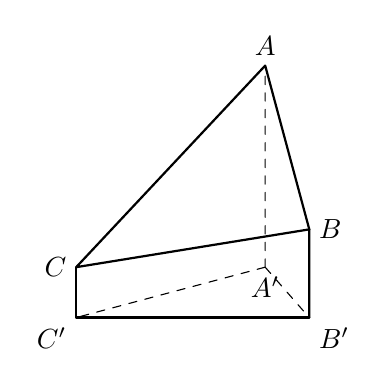
\begin{tikzpicture}[line cap=round,line join=round,scale=0.8]
\usetikzlibrary{calc}

% --- ground plane A'B'C' as a parallelogram ---
\coordinate (Cp) at (0,0);
\coordinate (Bp) at (3.7,0);
\coordinate (Ap) at (3.0,0.8);

\draw[thick]   (Bp) -- (Cp) -- cycle;

% labels on plane
\node[below left]  at (Cp) {$C'$};
\node[below right] at (Bp) {$B'$};
\node[below]       at (Ap) {$A'$};

% --- verticals up to A,B,C ---
\def\hA{3.2}
\def\hB{1.4}
\def\hC{0.8}

\coordinate (A) at ($(Ap)+(0,\hA)$);
\coordinate (B) at ($(Bp)+(0,\hB)$);
\coordinate (C) at ($(Cp)+(0,\hC)$);

\draw[dashed] (Ap) -- (A);
\draw[thick] (Bp) -- (B);
\draw[thick] (Cp) -- (C);

% --- triangle ABC in space ---
\draw[thick] (A) -- (B) -- (C) -- cycle;

% --- some auxiliary dashed lines on the plane (to mimic the sketch) ---
\draw[dashed] (Ap) -- (Bp);
\draw[dashed] (Ap) -- (Cp);

% labels of A,B,C
\node[above] at (A) {$A$};
\node[right] at (B) {$B$};
\node[left]  at (C) {$C$};
\end{tikzpicture} (\hspace{1cm})
\begin{choices}
\choice{{$346$}}
\choice{{$373$}}
\choice{{$446$}}
\choice{{$473$}}
\end{choices}
\end{problem}

\begin{answer}

\end{answer}

\begin{solutions}

\end{solutions}